\subsection{Round-Robin (RR)}
RR es un algoritmo de los más viejos, simple, justo y ampliamente usado.

A cada proceso se le asigna un tiempo (quantum) durante el cuál le es permitido correr.
Si el proceso sigue corriendo al final del quantum, los recursos le son quitados y se le da paso a otro proceso.
Si el proceso se bloquea, pierde el quantum que le quedaba y los recursos son dados a otro proceso.

Implementar RR es simple, sólo se requiere una lista de procesos 'Ready'.
Cuando el proceso usa su quantum es puesto al final de la lista. 
Si éste se bloquea, es removido de dicha lista y volverá a ser agregado en cuanto se desbloquee.

En nuestro caso usamos las siguientes estructuras de datos:
 \begin{description}
  \item[Cola de procesos 'Ready']{}
 \end{description}

\begin{algorithm}
 \caption{Round-Robin}
 \begin{algorithmic}[1] 
 \Procedure{load}{$pid$}
   \State{encolo la nueva tarea en readyTasks}
 \EndProcedure


 \Procedure{unblock}{$pid$}
   \State{encolo la tarea desbloqueada en readyTasks}
 \EndProcedure


 \Procedure{tick}{$cpu,\ motivo$}
   \If{el cpu esta ejecutando IDLE}
      \State{llamo a NEXT(cpu) para obtener la próxima tarea a ejecutar}
   \Else
      \If{el motivo es un TICK}
	 \State{Actualizo el quantum}
	 \If{se termino el quantum}
	    \State{encolo la tarea en readyTasks}
	    \State{renuevo el quantum}
	    \State{llamo a NEXT(cpu) para obtener la próxima tarea a ejecutar}
	 \EndIf	    
      \ElsIf{el motivo es un BLOCK o un EXIT}
	  \State{renuevo el quantum}
	  \State{llamo a NEXT(cpu) para obtener la próxima tarea a ejecutar}	
      \EndIf
   \EndIf
 \EndProcedure

 
 \Procedure{next}{$cpu$}
    \If{hay tareas esperando en readyTasks}
	\State{retornar la primera de la cola readyTasks y quitarla}
    \Else
	\State{retornar IDLE}
    \EndIf
 \EndProcedure
 \end{algorithmic}
\end{algorithm}

Para las simulaciones mantuvimos los siguientes costos:
\begin{description}
 \item[costo de cambio de contexto = 1 :]{En un CPU real se deben intercambiar estructuras de datos que contienen información de los procesos antes de poder correr la nueva tarea.}
 \item[costo de migración de núcleo = 2 :]{Se deben intercambiar las mismas estructuras de datos que para el cambio de contexto pero la 'distancia' del caché de un núcleo al de otro es mayor que dentro de sí mismo.}
\end{description}

Correremos un par de lotes de tareas para verificar que el comportamiento del scheduler es el esperado.

\begin{center}
 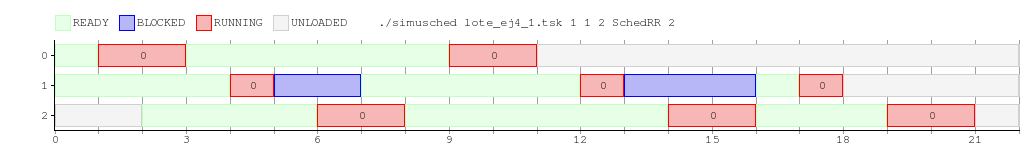
\includegraphics[scale=0.48]{./RR/RR_simple.png}
\end{center}

Se puede observar que no es un algoritmo FCFS porque, en principio, hace desalojo de tareas cada cierto quantum.
Además las tareas que se bloquean son desalojadas de inmediato, sin encolarlas en ReadyTasks hasta que se desbloqueen.

\begin{center}
 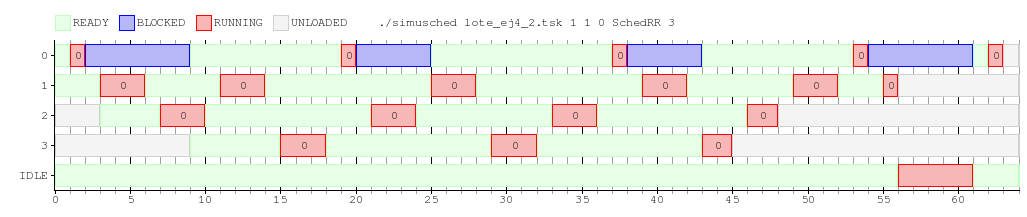
\includegraphics[scale=0.48]{./RR/RR_example_2.png}
\end{center}

Se puede ver que el proceso 0 es desalojado en cuanto se bloquea, cediendo el procesador al
proceso 1 (siguiente en la cola de ReadyTasks).\\
En cuanto el proceso 1 termina su quantum es desalojado (y movido al final de la cola de ReadyTasks).
Y se deja correr el proceso 2.\\

Entre los ciclos 14 y 15, la cola de ReadyTasks tiene la siguiente forma:
[3, 2, 0, 1].\\
Ya que el proceso 0 fue desencolado en cuanto se bloqueó, y vuelto a encolar en el
ciclo 11 (cuando se desbloquea), antes de que termine el quantum del proceso 1.\\

Veamos ahora un ejemplo de una mala elección de quantum para un entorno donde el
costo de cambio de contexto es elevado.

\begin{center}
 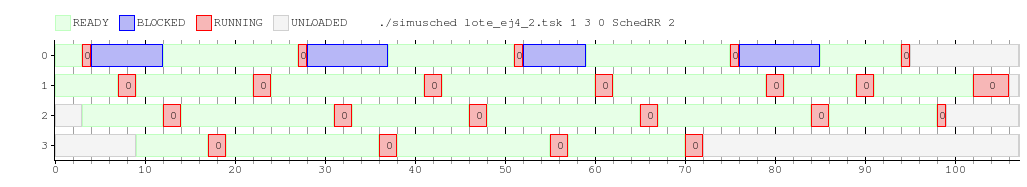
\includegraphics[scale=0.48]{./RR/RR_example_3.png}
\end{center}

Como se puede observar, tarda 106 ciclos en completar la ejecución del lote de tareas.
A diferencia del anterior (que tardaba 63 ciclos).

Esto se debe a que el procesador está más tiempo haciendo tareas de mantenimiento (cambio de contexto)
que efectivamente ejecutando procesos.